\chapter{Theory}

Two of the studies presented within this thesis are for prospective measurements looking at the $H\rightarrow WW$ branching ratio and the forward-backward asymmetry in \ttbar~ production at CLIC during the 1.4~TeV stage. As such it is important to first examine the significance of these measurements in the context of the physics programme of CLIC and the wider state of particle physics.


\section{The Standard Model}

\begin{figure}
  \centering
  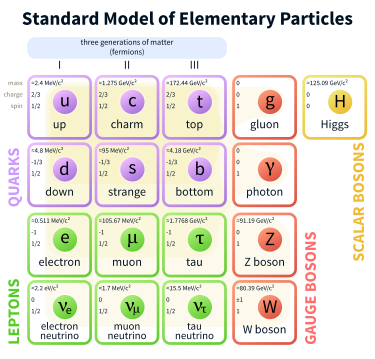
\includegraphics[width=0.55\textwidth,keepaspectratio]{Theory/fig/smparticles.png}
  \caption[Particles of the Standard Model]{Particles of the Standard Model}
  \label{fig:smparticles}
\end{figure}

The \ac{SM} is a quantum field theory representing our best current description of fundamental particles and the interactions between them. It consists of twelve spin-$\frac{1}{2}$ fermions (and their corresponding antiparticles), five spin 1 gauge bosons and one spin 0 scalar boson (as shown in \reffig{fig:smparticles}) where the interactions of the model are described by an $SU(3)_{C}\oplus SU(2)_{L}\oplus SU(1)_{Y}$ local gauge symmetry. The model describes pointlike particles which interact via the strong, weak and electromagnetic forces. No gravitational interactions are described within the model.

The fermions of the model can be classified into two families- leptons and quarks- according to how they interact. The quark family consists of the up(u), down(d), charm(c), strange(s), top(t) and bottom(b) quarks, all of which are capable of interacting via the strong, weak and electromagnetic force. The lepton family, consisting of the electron(e), muon($\mu$), tau($\tau$), electron neutrino($\nu_{e}$), muon neutrino($\nu_{\mu}$) and tau neutrino($\nu_{tau}$), are defined by the fact they carry no colour charge and so are incapable of interacting via the strong force, however they are still all capable of interacting via the weak force and the $e$/$\mu$/$\tau$ can interact electromagnetically. The gauge bosons are the mediators for the three fundamental forces of the model. The photon is a massless boson that mediates the electromagnetic force by coupling to particles with electrical charge. The gluon is also massless and mediates the strong force by coupling to particles with colour charge. The gluon is unique amongst the gauge bosons in that it is the only boson that carries the charge to which it couples (i.e. it is coloured) and so couples to itself. One direct consequence of this is that it is impossible to form a stable coloured state due to colour confinement and so quarks are only observed in net-colourless states called hadrons. When a quark is produced in an interaction, it will typically undergo a process known as hadronization in which the quark will bind to quarks/antiquarks spontaneously produced from the vacuum to form quark-antiquark pairs known as mesons or triplets of quarks or antiquarks known as baryons. The only exception to this is the top quark which will typically decay in a shorter timescale than is needed for hadronization to occur. The final three gauge bosons are the Z, W$^+$ and W$^-$ which are all massive and mediate the weak interaction via their coupling to weak isospin.

Much like the fermions can be separated into quarks and leptons according to the way the interact, the underlying symmetry of the \ac{SM} of $SU(3)_{C}\oplus SU(2)_{L}\oplus SU(1)_{Y}$ can be decomposed into separate parts according to the interactions that the symmetries describe. The $SU(3)_{C}$ represents transformations of the colour state of a system and so describes interactions involving the strong force. These interactions are commonly referred to as \ac{QCD}. The $SU(2)_{L}\oplus SU(1)_{Y}$ symmetry represents electroweak theory- a unified description of the weak and electromagnetic interactions. In this description, fermions can be thought of as consisting of left and right handed fields, where the left handed components transform as doublets under SU(2) transformations while the right handed components only transform as singlets. The result of this is that the weak interaction only acts on the left handed fields components. Hence the weak force only couples to left(right) handed particles(antiparticles.) 

One of the most interesting features of electroweak theory occurs when considering the effect of gauge transformations on the Lagrangian of the system. In quantum field theory, fermions can be descibed by a dirac field with the following Lagrangian:

\begin{equation}
  \label{eq:diracLagrangian}
\mathscr{L}=i\bar{\psi} \gamma^{\mu} \partial{\mu} \psi  -m\bar{\psi}\psi
\end{equation}

Applying a global phase transition of the form:

\begin{equation}
\psi \rightarrow \psi ' = e^{i\alpha}\psi
\end{equation}

will leave the Lagrangian unchanged due to the fact $e^{i\alpha}\psi e^{-i\alpha}\psi=1$. However, in the case of local gauge transformations where $e^{i\alpha}\psi \rightarrow  e^{i\alpha(\textbf{x})}\psi$, i.e. the phase has a local space-time dependence, then eq\refeq{eq:diracLagrangian} is no longer invariant:

\begin{equation}
\mathscr{L}=i\bar{\psi} \gamma^{\mu} \partial{\mu} \psi  -m\bar{\psi}\psi -\bar{\psi}(\textbf{x})\gamma^{\mu}\partial{\mu}\alpha(\textbf{x})
\end{equation}

In order to restore the invariance, the derivative $\partial{\mu}$ must be replaced with the covariant derivative $D_{\mu}$ which is of the form:

\begin{equation}
  D_{\mu}=\partial{\mu}+ieA_{\mu}
\end{equation}

where $A_{\mu}$ is a gauge field which transforms as:

\begin{equation}
  A_{\mu}\rightarrow A_{\mu}^{'} = A_{\mu} - \frac{1}{e}\partial{\mu}\alpha(\textbf{x})
\end{equation}

In electroweak theory the gauge fields required are found to consist of three weak isospin fields, $W_1, W_2 and W_3$,  coming from the SU(2) group and one eak hypercharge field ,B, from U(1). The interesting result of this is the prediction that the bosons associated with these fields and the fermions they interact with to be massless, however this is experimentally found to be false as the bosons of the weak force, Z and W, have masses of 91.876 $\pm$ 0.0021 GeV and 80.385 $\pm$ 0.015 GeV respectively. Furthermore, in electroweak theory it can be shown that the presence of massive electroweak bosons results in unphysical predictions in the \ac{SM} e.g. violation of unitarity when calculating the amplitude of $WW\rightarrow WW$ scattering (REFERENCE). These problems can be fixed by via consideration of the final particle within the \ac{SM}, the Higgs boson.


\section{The Higgs Boson and the Origin of Mass}

To solve the problems seen in the electroweak sector, Brout, Englert and Higgs (REFERENCE) proposed that mass terms could be generated within the \ac{SM} via the addition of a complex, scalar doublet of the group $SU(2)_{L}$ pssessing four degrees of freedom:

\begin{equation}
\phi = \begin{pmatrix} \phi^{+} \\ \phi^{0} \end{pmatrix} 
\end{equation}

with potential:

\begin{equation}
V(\phi) = \mu^{2}\phi^{\dagger}\phi + \frac{\lambda^{2}}{2}(\phi^{\dagger}\phi)^{2}
\end{equation}

The Higgs field is found to interact with the $W_{1},W_{2},W_{2}$ and $B$ gauge fields. In the case that $\mu^{2}<0$, due to the Higgs field acquiring a non-zero expectation value, the $SU(2)_{L}\oplus SU(1)_{Y}$ symmetry is found to break leaving only a $U(1)_{em}$ symmetry corresponding to a massless photon. Of the four degrees of freedom associated with the Higgs field, the interaction of the field with the W and B gauge fields results in three massive gauge bosons corresponding to the measured $Z$ and $W^{\pm}$ masses, where the physically observed bosons actually represent mixtures of the underlying gauge fields:

\begin{equation}
\gamma = \cos\theta_{W}B  +\sin\theta_{W}W_{3} 
\end{equation}

\begin{equation}
Z = \cos\theta_{W}W_{3}  -\sin\theta_{W}B
\end{equation}

\begin{equation}
W^{\pm}= \frac{1}{\sqrt{2}}(W_{1}\mp iW_{2})
\end{equation}

Where $\theta_{W}$ is the weak mixing angle which depends on g ang g$'$.

The last remaining degree of freedom of the Higgs field corresponds to the Higgs boson itself. The mass of the Higgs boson can be determined to be $m_{H}=\sqrt{2\lambda}\nu$, where $\lambda$ is the Higgs self coupling parameter and $\nu$ is the vacuum expectation value for the Higgs field. While $\nu$ can be calculated within the standard model, $\lambda$ is a free parameter and so the mass of the Higgs is not derivable. Experimentally it is found to be $\sim$125GeV.

While the mass of the Higgs is of interest as it represents a free parameter in the standard model, there are many more properties of the Higgs that are important to measure. In particular the way in which theHiggs boson couples to other particles is well predicted within the \ac{SM} and is expected to vary between various \ac{BSM} models. Within the \ac{SM} the coupling of the Higgs to fermions and bosons is diferent but depends on mass in each case:


\begin{equation}
g_{Hf\bar{f}}=\frac{M_f}{\nu} ~~~~~~~~    g_{HBB}=\frac{2M_B^2}{\nu} 
\end{equation}

Due to this clear mass dependence, a fit of the coupling to each fermion as a function of the fermions mass represents a powerful way of testing the \ac{SM}. The mass dependence on the Higgs couplings also presents a new way to perform direct searches for new physics involving as yet unseen massive particles by looking at the branching ratio of Higgs decays to invisible decay products and the total Higgs decay width. This is of particluar interest in searches for dark matter which is known to interact gravitationally and so must possess mass. 

\section{Higgs Measurements at CLIC}
\begin{figure}
  \centering
  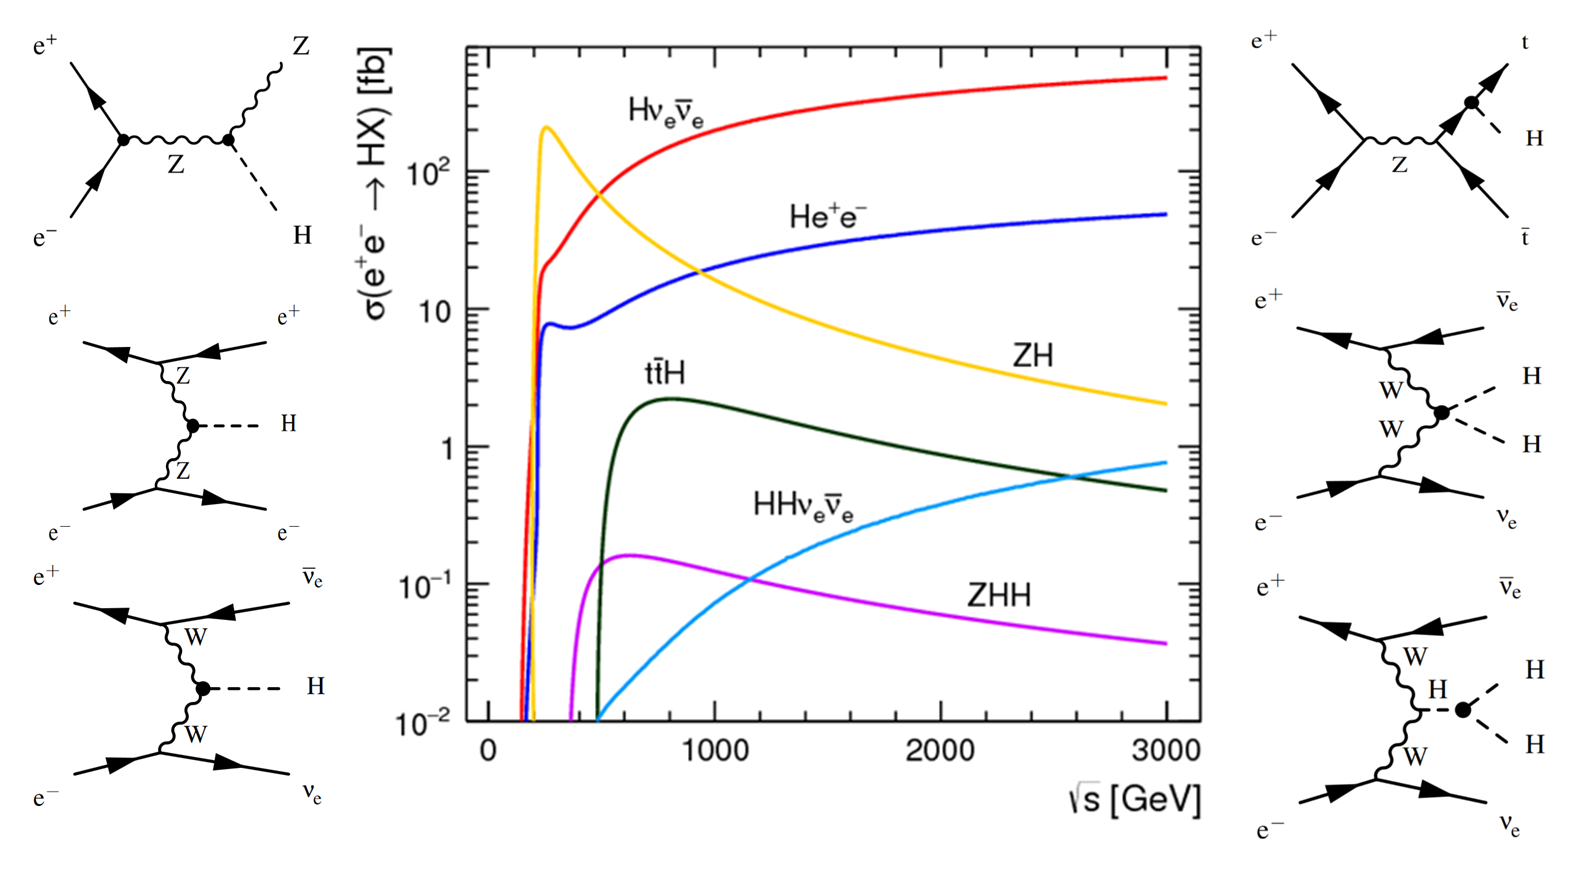
\includegraphics[width=0.95\textwidth,keepaspectratio]{Theory/fig/HiggsProcessesExtra.png}
  \caption[Cross Sections For Higgs Production Mechanisms]{Cross Sections For Higgs Production Mechanisms}
  \label{fig:higgsXSecs}
\end{figure}

The CLIC physics programme has a large focus on characterising the Higgs boson due to the large uncertainties on many of it's associated properties relative to other sectors of the standard model. In particluar it will aim to measure the mass, width, and couplings of the Higgs in a model independent manner. Electron positron collisions provide access to numerous Higgs production mechanisms which can be seen in \ref{fig:higgsXSecs}. Due to the strong energy dependence on many of the cross sections on energy, different processes will be of interest at each of the three energy stages operated at CLIC. At 380GeV the focus will predominantly be on measuring the Higgsstrahlung ($ZH$) process in which a Z boson radiates a Higgs boson, while at higher energies vector boson fusion ($H\nu\nu,Hee$) dominates and new processes such as di-Higgs production become accessible. A summary of all the results from current Higgs studies performed by CLIC is available in \cite{Abramowicz:2016zbo}.

\subsection{Higgsstrahlung}

\begin{figure}
  \centering
  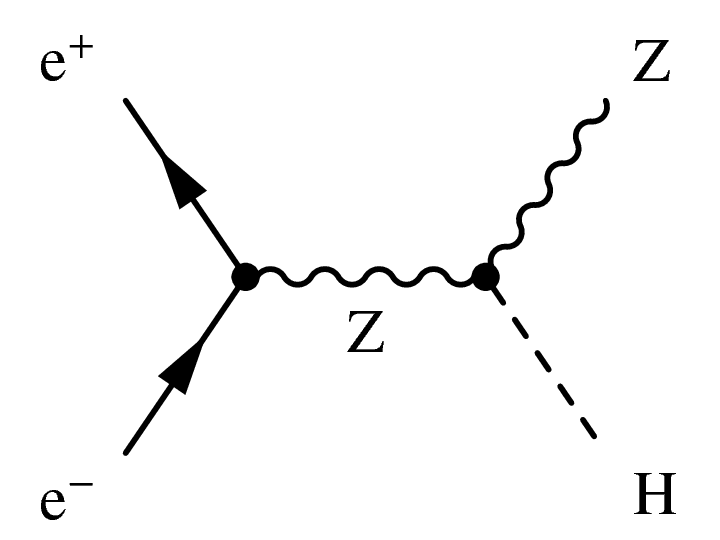
\includegraphics[width=0.45\textwidth,keepaspectratio]{Theory/fig/HiggsStrahlung.png}
  \caption[The Higgstrahlung Process]{The Higgstrahlung Process}
  \label{fig:higgsstrahlung}
\end{figure}


One of the key aims of the experiment will be to examine the Higgsstrahlung process shown in \ref{fig:higgsstrahlung}. In this process, if the four momentum of the Z boson can be measured to high precision, then because the initial conditions of the collision are well known, one can determine the mass of the particle it is recoling against ($m_{rec}^{2} = s + m_{z}^{2} - 2E_{z}^{2}$) and infer the presence of the Higgs. This allows properties such as the Higgs mass, cross-section and coupling to the Z to be measured without actually ever measuring the decay products of the Higgs boson which in turn allows the measurements to be model independent as few assumptions must be made about the interactions of the Higgs. This method is not possible at hadron colliders such as the LHC where, even though the Higgsstrahlung process still occurs, as the four momentum of the colliding particles can never be known to as high a level of precision due to their composite nature. Using the clean signal from cases where the Z decays to a pair of muons or electrons it is possible to measure the recoil mass to high precision and thus determine the mass of the Higgs to $\Delta m_{H} = 110~MeV$ (see figure \ref{fig:higgsmass} using data from the low energy stage only. This value can be further improved to $\Delta m_{H} = 44~MeV$ when including direction measurement results from the $ee\rightarrow H\nu\bar{\nu}, H\rightarrow b\bar{b}$ channel at 3~TeV. Despite giving a poorer resolution on the Z four momentum, the $Z\rightarrow qq$ higgsstrahlung channel is also considered due to it's larger cross section. Using this channel a limit of $BR(H\rightarrow invis.) <0.97\%$ at 90\% C.L. can be set. 

\begin{figure}
  \centering
  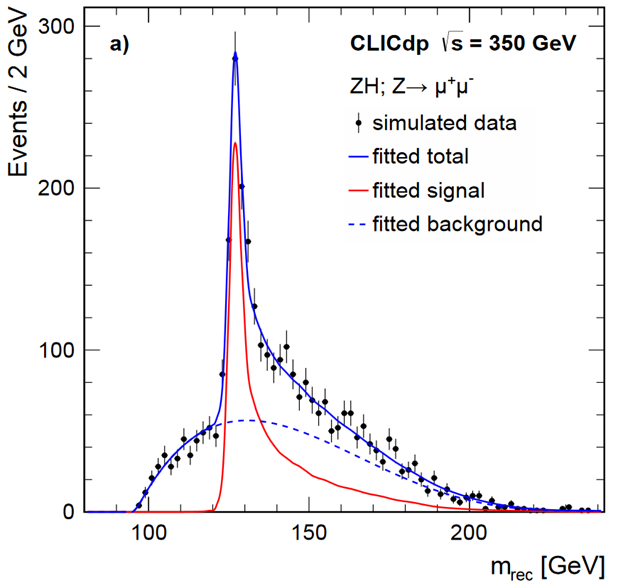
\includegraphics[width=0.45\textwidth,keepaspectratio]{Theory/fig/HiggsRecoilMass.png}
  \caption[Reconstructed recoil mass from Higgsstralung process]{Reconstructed recoil mass from Higgsstralung process}
  \label{fig:higgsstrahlung}
\end{figure}

 
\subsection{Model Independent Extraction of Higgs Couplings}


While the Higgsstrahlung alone allows the mass and branching ratios of the Higgs to be determined, by measuring the rates of several different Higgs processes and combining them in the right ratio, it is further possible to extract the absolute width of the Higgs. One such ``recipe'' proposed for doing this is shown in \ref{modelindependentformula} \cite{Durig:2014lfa}:

\begin{equation}
  \label{modelindependentformula}
  \Gamma_H = \frac{Y_1^2Y_3^2}{Y_4^2Y_2}
\end{equation}

where

\begin{equation}
X_1=\sigma_{ZH} \propto g_{HZZ}^2
\end{equation}

\begin{equation}
  \label{X2}
  X_2=\sigma_{H\nu\bar{\nu}} \times BR(H\rightarrow WW^*) \propto \frac{g_{HWW}^4}{\Gamma_H}
\end{equation}

\begin{equation}
X_3=\sigma_{H\nu\bar{\nu}} \times BR(H\rightarrow b\bar{b}) \propto \frac{g_{HWW}^{2}g_{Hbb}^2}{\Gamma_H}
\end{equation}

\begin{equation}
X_4=\sigma_{ZH} \times BR(H\rightarrow b\bar{b}) \propto \frac{g_{HZZ}^{2}g_{Hbb}^2}{\Gamma_H}
\end{equation}


Currently at the LHC the standard process for extracting couplings from the equivalent measurements of $X_{2,3\&4}$ is to multiply through by the standard model value of the Higgs width. This type of measurement is referred to as `model-dependent` as the values determined for the Higgs couplings carry the implicit assumption that the standard model is correct in it's prediction of the Higgs width. At CLIC, because the width can be measured experimentally there is no need to make this assumption and so the couplings are measured in a ``model-independent'' way. The unique ability of linear colliders to perform model-independent measurements is one of the largest driving factors for constructing and using them as a so called ``Higgs-Factory''. One limiting factor for the model-independent measurements of the couplings is that they are always ultimately dependent on the precision to which the ZH cross section can be measured (predicted to be $\Delta h_{HZZ} = 0.8\%$) as this quantity is always needed in the ratio used to extract $\Gamma_H$. With the exception of $X_1$, the choice of variables used is not unique (e.g. one could replace the production mechanism in $X_1$ and $X_2$ with ZZ-fusion rather than WW-fusion,) however the combination shown here is expected to give the highest precision on $\Gamma_H$ due to the large cross-section associated with WW-fusion and the high branching ratio of $H\rightarrow b\bar{b}$ ($\sim$ 65\%). In chapter \ref{Higgs Analysis} we will present our research on the precision to which $X_2$ can be measured during the 1.4~TeV run at CLIC.

\begin{figure}
\centering
\begin{subfigure}{.5\textwidth}
  \centering
  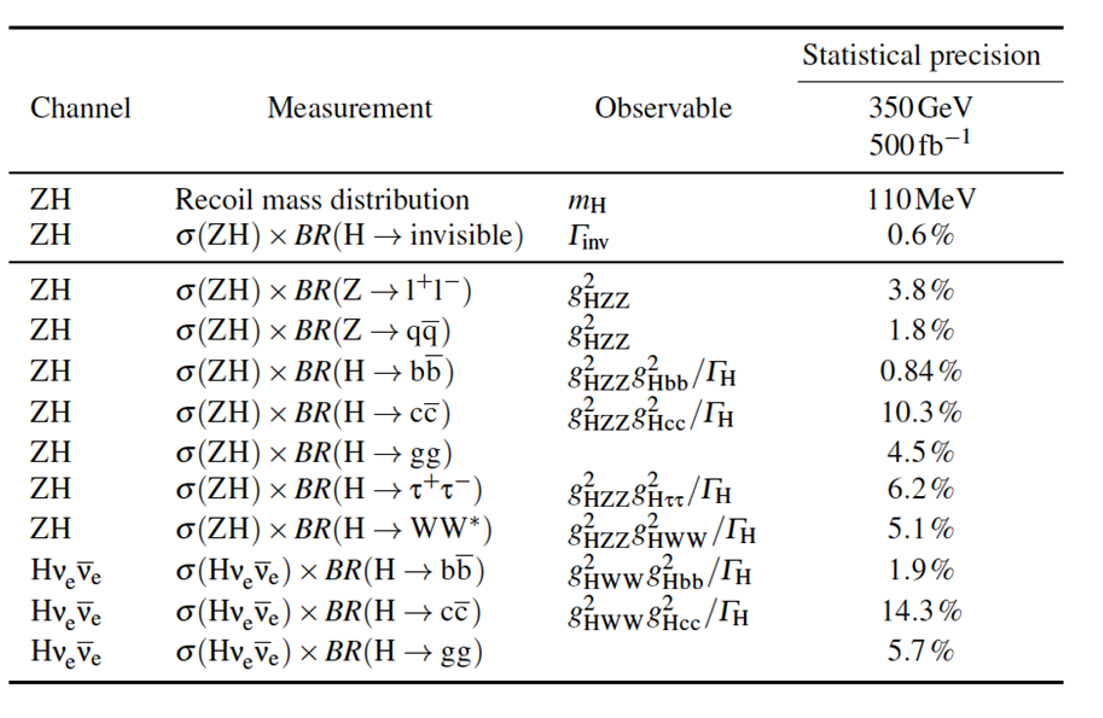
\includegraphics[width=.4\linewidth]{Theory/fig/table28_350GeVPrecisions}
 % \caption{}
  \label{fig:350GeVNumbers}
\end{subfigure}%
\begin{subfigure}{.5\textwidth}
  \centering
  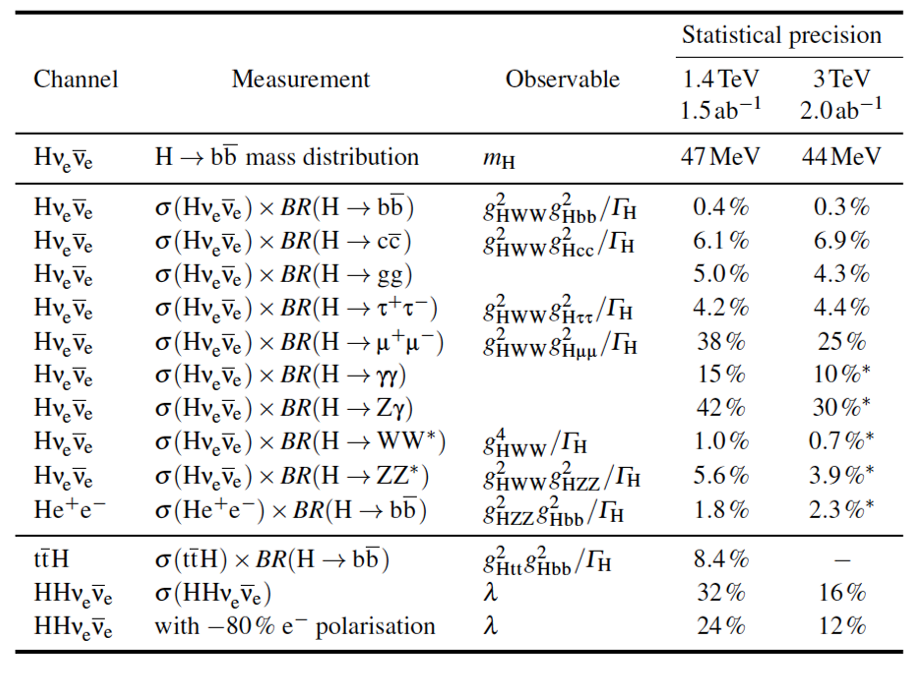
\includegraphics[width=.4\linewidth]{Theory/fig/table29_HighEPrecisions}
 % \caption{}
  \label{fig:HighENumbers}
\end{subfigure}
\caption[Expected statistical uncertainties for Higgs related measurments at CLIC for the nominal luminosity at each of the proposed energy stages assuming unpolarised beams]{Expected statistical uncertainties for Higgs related measurments at CLIC for the nominal luminosity at each of the proposed energy stages assuming unpolarised beams}
\end{figure}

\begin{figure}
\centering
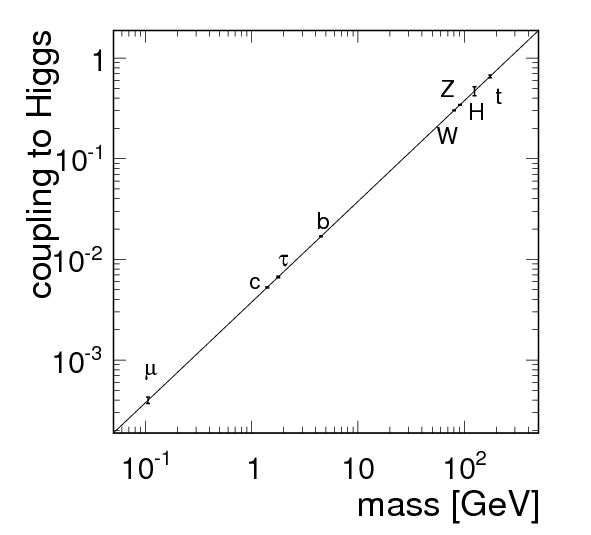
\includegraphics[width=.4\linewidth]{Theory/fig/HiggsCouplings}
\caption[Expected precision on model independent measurements of the Higgs couplings]{Expected precision on model independent measurements of the Higgs couplings}
\label{fig:modelIndependentCouplings}
\end{figure}


In practice it is expected that an 11 parameter global fit to multiple variations of these measurements will be performed at each stage of operation to extract the Higgs width and it's couplings to both fermions and bosons. The relevant inputs for these fits are shown in tables \ref{fig:350GeVNumbers}\ref{fig:HighENumbers} while the results of the fits are shown in \reffig{fig:modelIndependentCouplings}

For context it is also important to compare these results to what can be expected from current leading experiments such as ATLAS and CMS at the LHC and the predicted precision they will have optained by the time CLIC would begin operation. Because the Higgs width can not be explicitly calculated at Hadron colliders, it is best to compare the model dependent version of the CLIC analysis with those predicted by ATLAS and CMS. In this situation, becuase the precision of the couplings is no longer limited by the precision on $g_{HZZ}$ the predicted precision for CLIC is seen to improve considerably. One can see from figure (SHOW CLIC MODEL DEPENDENT PLOT AND LHC PREDICTIONS) that in almost all cases CLIC is expected to provide a considerable improvement over what can be achieved at the LHC with many of the key parameters associated with the Higgs being measured to sub percent precision.

Ultimately the aim of performing precision measurements is to be allow the validation or rejection of theoretical models. While the results seen so far at the LHC suggest that the observed Higgs Boson is that of the \ac{SM}, their are numerous alternative theories that predict a Higgs like particle with properties similar to what has been observed but which differ to a degree not yet measureable by current experiments. The details of these theories will not be expanded upon within this thesis, however the deviations expected in the Higgs couplings of these theories relative to the \ac{SM} are shown in table (INSERT SNOWMASS TABLE.) These values should only be taken as a rough guideline for the precision required to discover/reject the theories as they are based on the assumption that new physics occurs at a specific scale (in this case 1~TeV,) however it is clear that the level of precision required to provide sensitivity to these models will be greater than what will be possible with the LHC but could be within the scope of the proposed CLIC physics programme.  


\section{Top Quark Physics}

Highest mass in the standard model, not precisely measured, possible sensitivity to BSM physics.

CLIC has a rich program of top physics thanks to it's operation at 380~GeV close to the top pair production threshold.

Beyond the mass and width of the top, one of the key aims will be to measure the coupling of of the top to z/gamma. Provides access to form factors that are sensitive to BSM effects.

Several measurements necessary such as the AFB and cross section

Define what the forward backward asymmetry is, brief history of measurements elsewhere

How it fits in with the calculation of the EW couplings

New physics that can effect these couplings e.g. Z'

